

\documentclass[man,floatsintext]{apa6}
\usepackage{lmodern}
\usepackage{amssymb,amsmath}
\usepackage{ifxetex,ifluatex}
\usepackage{fixltx2e} % provides \textsubscript
\ifnum 0\ifxetex 1\fi\ifluatex 1\fi=0 % if pdftex
  \usepackage[T1]{fontenc}
  \usepackage[utf8]{inputenc}
\else % if luatex or xelatex
  \ifxetex
    \usepackage{mathspec}
  \else
    \usepackage{fontspec}
  \fi
  \defaultfontfeatures{Ligatures=TeX,Scale=MatchLowercase}
\fi
% use upquote if available, for straight quotes in verbatim environments
\IfFileExists{upquote.sty}{\usepackage{upquote}}{}
% use microtype if available
\IfFileExists{microtype.sty}{%
\usepackage{microtype}
\UseMicrotypeSet[protrusion]{basicmath} % disable protrusion for tt fonts
}{}
\usepackage{hyperref}
\hypersetup{unicode=true,
            pdftitle={Assessing sampling methods for generalization from RCTs: Modeling recruitment and participation},
            pdfauthor={Gleb Furman~\& James E. Pustejovsky},
            pdfborder={0 0 0},
            breaklinks=true}
\urlstyle{same}  % don't use monospace font for urls
\usepackage{graphicx,grffile}
\makeatletter
\def\maxwidth{\ifdim\Gin@nat@width>\linewidth\linewidth\else\Gin@nat@width\fi}
\def\maxheight{\ifdim\Gin@nat@height>\textheight\textheight\else\Gin@nat@height\fi}
\makeatother
% Scale images if necessary, so that they will not overflow the page
% margins by default, and it is still possible to overwrite the defaults
% using explicit options in \includegraphics[width, height, ...]{}
\setkeys{Gin}{width=\maxwidth,height=\maxheight,keepaspectratio}
\IfFileExists{parskip.sty}{%
\usepackage{parskip}
}{% else
\setlength{\parindent}{0pt}
\setlength{\parskip}{6pt plus 2pt minus 1pt}
}
\setlength{\emergencystretch}{3em}  % prevent overfull lines
\providecommand{\tightlist}{%
  \setlength{\itemsep}{0pt}\setlength{\parskip}{0pt}}
\setcounter{secnumdepth}{0}
% Redefines (sub)paragraphs to behave more like sections
\ifx\paragraph\undefined\else
\let\oldparagraph\paragraph
\renewcommand{\paragraph}[1]{\oldparagraph{#1}\mbox{}}
\fi
\ifx\subparagraph\undefined\else
\let\oldsubparagraph\subparagraph
\renewcommand{\subparagraph}[1]{\oldsubparagraph{#1}\mbox{}}
\fi

%%% Use protect on footnotes to avoid problems with footnotes in titles
\let\rmarkdownfootnote\footnote%
\def\footnote{\protect\rmarkdownfootnote}


  \title{Assessing sampling methods for generalization from RCTs: Modeling recruitment and participation}
    \author{Gleb Furman\textsuperscript{1}~\& James E. Pustejovsky\textsuperscript{1}}
    \date{}
  
\shorttitle{Assessing sampling methods for generalization from RCTs}
\affiliation{
\vspace{0.5cm}
\textsuperscript{1} University of Texas at Austin}
\usepackage{csquotes}
\usepackage{upgreek}
\captionsetup{font=singlespacing,justification=justified}

\usepackage{longtable}
\usepackage{lscape}
\usepackage{multirow}
\usepackage{tabularx}
\usepackage[flushleft]{threeparttable}
\usepackage{threeparttablex}

\newenvironment{lltable}{\begin{landscape}\begin{center}\begin{ThreePartTable}}{\end{ThreePartTable}\end{center}\end{landscape}}

\makeatletter
\newcommand\LastLTentrywidth{1em}
\newlength\longtablewidth
\setlength{\longtablewidth}{1in}
\newcommand{\getlongtablewidth}{\begingroup \ifcsname LT@\roman{LT@tables}\endcsname \global\longtablewidth=0pt \renewcommand{\LT@entry}[2]{\global\advance\longtablewidth by ##2\relax\gdef\LastLTentrywidth{##2}}\@nameuse{LT@\roman{LT@tables}} \fi \endgroup}

\begin{document}
\maketitle

\hypertarget{results}{%
\section{Results}\label{results}}

\hypertarget{generalizability}{%
\subsection{Generalizability}\label{generalizability}}

Figure \ref{fig:fig-SMD-by-Var} displays the average SMD between the samples and the population for each covariate and at each population participation rate resulting from each sampling method. The dotted horizontal line indicates a cutoff of .25, where SMDs above that indicate large differences between the sample and population for that covariate. Stratified methods consistently performed better than unstratified methods. SBS generally performed as well as or better than SRS. URS often resulted in highly unrepresenative samples except in cases where population participation rates were extremely high.

Figure \ref{fig:fig-avg-Bindex} displays the average \(B\)-index for each method across participation rates. At population participation rates of 60\% and higher, all methods resulted in similarly generalizable samples. However, at lower rates only SBS and SRS consistantly generated highly generalizable samples. SCS and URS performed equally, while UCS resulted in relatively less generalizable samples.

\begin{figure}
\centering
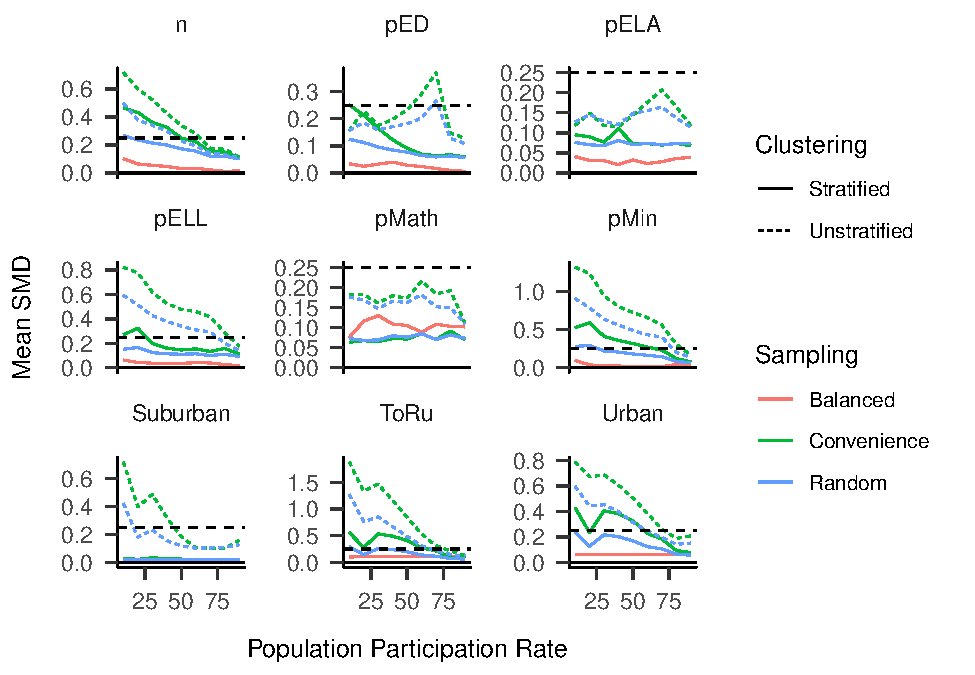
\includegraphics{GenSamp_Results_files/figure-latex/fig-SMD-by-Var-1.pdf}
\caption{\label{fig:fig-SMD-by-Var}Averge Standardized Mean Differences between sample and population}
\end{figure}

\begin{figure}
\centering
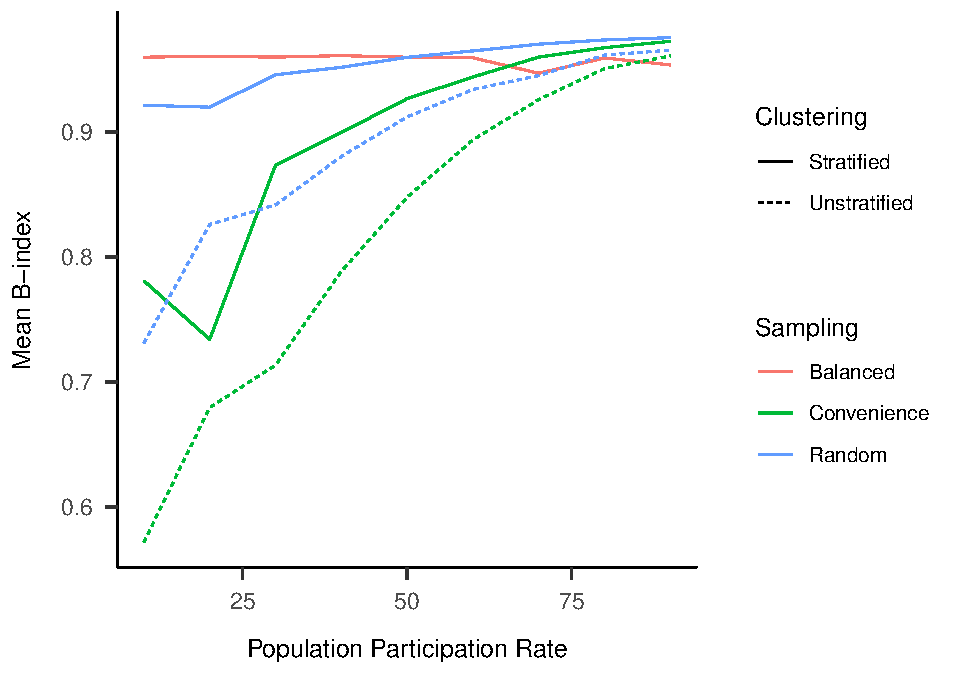
\includegraphics{GenSamp_Results_files/figure-latex/fig-avg-Bindex-1.pdf}
\caption{\label{fig:fig-avg-Bindex}Averge \(B\)-index across participation rates by sampling method}
\end{figure}

\hypertarget{feasibility}{%
\subsection{Feasibility}\label{feasibility}}

Figure \ref{fig:fig-units-contacted} reports the average number of schools that needed to be contacted before a full sample of \(N = 60\) schools was selected. At higher participation rates differences between methods were negligibile. However, as participation rates decreased the disparity between the methods became more apparent. Overall, UCS required the least \enquote{effort} to recruit a full sample, followed by URS and SCS, SRS, and finally SBS. Figure \ref{fig:fig-response-rates} plots the participation rates of schools approached for recruitment against the population participation rates. As expected, URS participation rates reflected those in the population. Both UCS and SCS resulted in higher participation rates, while SRS and SBS resulted in lower participation rates.

\begin{figure}
\centering
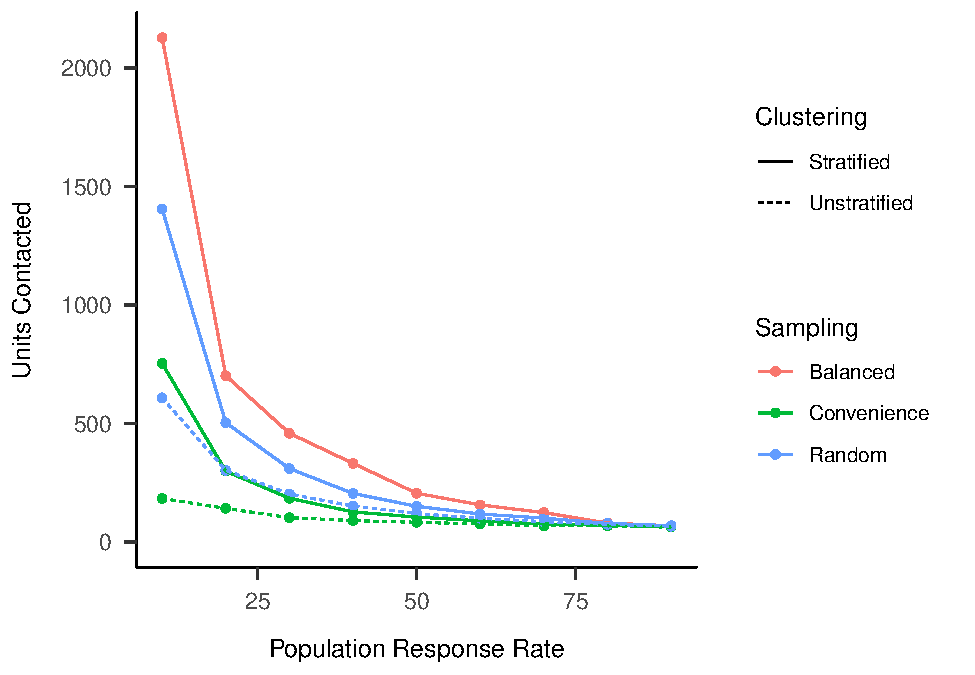
\includegraphics{GenSamp_Results_files/figure-latex/fig-units-contacted-1.pdf}
\caption{\label{fig:fig-units-contacted}Averge number of schools contacted to achieve N = 60}
\end{figure}

\begin{figure}
\centering
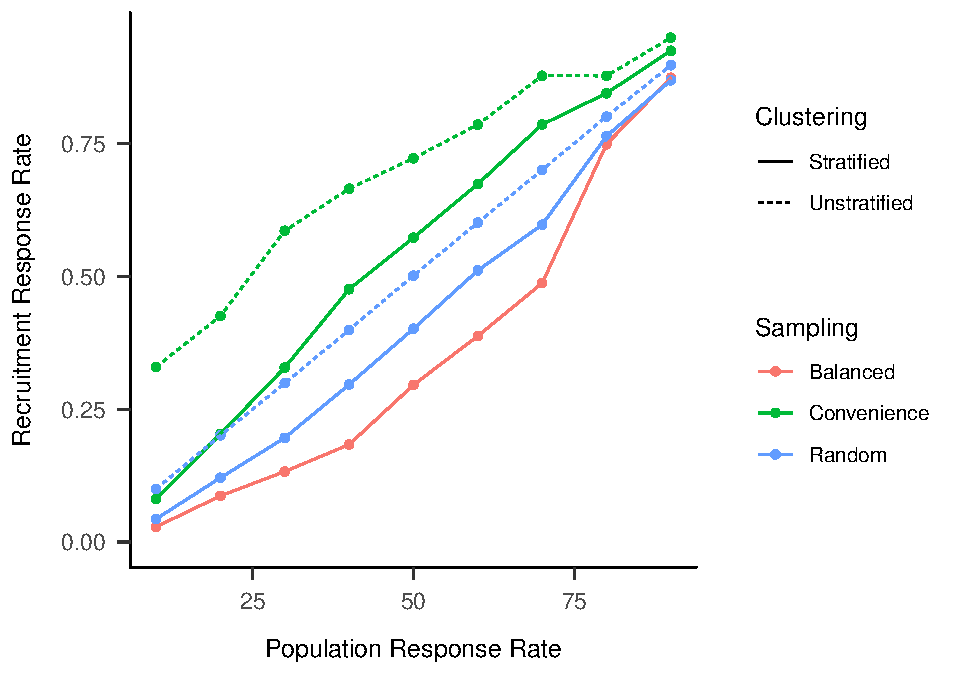
\includegraphics{GenSamp_Results_files/figure-latex/fig-response-rates-1.pdf}
\caption{\label{fig:fig-response-rates}Recruitment response rates for each sampling method}
\end{figure}

\newpage

\hypertarget{references}{%
\section{References}\label{references}}

\begingroup
\setlength{\parindent}{-0.5in}
\setlength{\leftskip}{0.5in}

\hypertarget{refs}{}

\endgroup


\end{document}
